%\newcommand{\filespath}{../../Style/}%  JANCL path

\documentclass[english,utf8]{./hermes-journal}
\usepackage[utf8]{inputenc}
% \journalName{year}{volume}{issue}
\ria{2012}{22}{1}

\firstpagenumber{9}
\let\chapter\section
\usepackage[ruled,algo2e]{algorithm2e}
\usepackage{mathtools}
\usepackage{subfigure}
\mathtoolsset{showonlyrefs=true}

\newcommand{\argmax}{\operatorname*{argmax}} %\operatorname* pour les op. pouvant admettre des limites...
\newcommand{\argmin}{\operatorname*{argmin}}
\newcommand{\diag}{\operatorname*{diag}}

\newcommand{\p}{\mathcal{P}}
\newcommand{\R}{\mathcal{R}}
\newcommand{\s}{\mathcal{S}}
\newcommand{\A}{\mathcal{A}}
\newcommand{\X}{\mathcal{X}}
\newcommand{\Y}{\mathcal{Y}}
\newcommand{\D}{\mathcal{D}}
\newcommand{\T}{\mathcal{T}}
\newcommand{\lc}{\mathcal{L}}
\newcommand{\E}{\mathbb{E}}
\newcommand{\prob}{\mathbb{P}}
\newcommand{\Mu}{\boldsymbol{\mu}}
%\newcommand{\Xi}{\boldsymbol{\xi}}


%\newtheorem{theorem}{Theorem}

% \title[short header title]{title}
\title[SCIRL]{Classification structurée pour l'apprentissage par renforcement}
\author[1,2]{Edouard}{Klein}
\author[2]{Bilal}{Piot}
\author[2,3]{Matthieu}{Geist}
\author[2,3]{Olivier}{Pietquin}


% addresses are automatically numbered
\address{LORIA -- team ABC\\
Nancy, France
}{}
\address{Supélec -- IMS-MaLIS Research Group\\
Metz, France}
        {prenom.nom@supelec.fr}
\address{ UMI 2958 (GeorgiaTech-CNRS)\\
Metz, France}{}

\abstract{  This paper adresses the inverse reinforcement learning (IRL) problem, that
  is inferring a reward for which a demonstrated expert behavior is
  optimal. We introduce a new algorithm, SCIRL, whose principle is to use
  the so-called feature expectation of the expert as the
  parameterization of the score function of a multi-class
  classifier. This approach produces a reward function for which the
  expert policy is provably near-optimal. Contrary to most of
  existing IRL algorithms, SCIRL does not require solving the
  direct RL problem. Moreover, with an appropriate heuristic, it can succeed with only trajectories sampled
  according to the expert behavior. This is illustrated on a car
  driving simulator.}
\resume{Cette contribution traite du problème de l'apprentissage par imitation par le biais de l'apprentissage par renforcement inverse (\emph{ARI}). Dans ce contexte, un expert accomplit une tâche qu'un agent artificiel doit essayer de reproduire. L'ARI part du postulat que l'expert optimise avec succès une fonction de récompense ; le problème consiste à deviner cette fonction à partir de  traces du comportement de l'expert. Les algorithmes d'ARI existants nécessitent une ou plusieurs des conditions suivantes pour fonctionner : trajectoires complètes de la part de l'expert, un modèle génératif pour les estimations de type Monte-Carlo, la connaissance des probabilités de transition, la capacité de résoudre le problème direct (celui de l'apprentissage par renforcement) de manière répétée ou l'accès à la strategie complète de l'expert. Notre contribution consiste en un nouvel algorithme d'ARI levant l'ensemble de ces contraintes. En utilisant une méthode supervisée dans laquelle nous introduisons implicitement la structure du processus décisionnel de Markov ({\it PDM}) sous-jacent, nous créons un algorithme basé sur une descente de sous-gradient, possèdant une faible complexité tant en échantillons que calculatoire et surtout ne nécessitant pas la résolution du problème direct.}

\keywords{Reinforcement Learning, Inverse Reinforcement Learning}
\motscles{Apprentissage par Renforcement, Apprentissage par Renforcement Inverse}


\begin{document}
\newtheorem{prop}[theorem]{Proposition}
\maketitle

\newpage

\section{Contexte et notations}
\label{sec:background}

\subsection{Apprentissage par Renforcement (Inverse)}
\label{subsec:background:irl}

Un Processus Décisionnel de Markov (PDM)~\cite{Puterman:1994} est un ensemble $\{\s,\A,\p,\R,\gamma\}$ avec $\s$ l'espace d'état fini\footnote{Cette contribution peut être étendue aux espaces d'état compacts moyennant le traitement de certains détails techniques.}, $\A$ l'espace d'action fini, $\p =
\{P_a = (p(s'|s,a))_{1\leq s,s'\leq |\s|}, a\in\A\}$ l'ensemble des probabilités de transition markoviennes, $\R\in\mathbb{R}^\s$ la fonction de récompense sur les états et $\gamma$ le facteur d'oubli.
Une politique déterministe $\pi\in\s^\A$ définit le comportement d'un agent. On quantifie la qualité de ce comportement par le biais de la fonction de valeur $v_\R^\pi\in\mathbb{R}^\s$ qui à chaque état associe la récompense pondérée cumulée recueillie par l'agent lorsqu'il part de cet état et suit la politique $\pi$ par la suite : $v_\R^\pi(s) = \E[\sum_{t\geq 0} \gamma^t \R(S_t)|S_0=s,\pi]$. Une politique optimale $\pi_\R^*$ (vis-à-vis de la fonction de récompense $\R$) est une politique dont la fonction de valeur $v^*_\R$ satisfait $v_\R^* \geq v_\R^\pi$, composante par composante, pour toute politique $\pi$.

Soit $P_\pi$ la matrice stochastique $P_\pi =
(p(s'|s,\pi(s)))_{1\leq s,s'\leq |\s|}$. Un léger abus de notation nous permet de nommer $a$ la politique associant l'action $a$ à chaque état $s$. Les opérateurs d'évaluation (resp. d'optimalité) de Bellman $T^\pi_\R\text{ (resp. $T^*_\R$)}:\mathbb{R}^\s
\rightarrow \mathbb{R}^\s$ sont définis par $T^\pi_\R v = \R + \gamma
P_\pi v$ and $T_\R^*v = \max_\pi T_\R^\pi v$.
%\begin{equation}
%  T^\pi_\R v = \R + \gamma P_\pi v \text{ and } T_\R^*v = \max_\pi T_\R^\pi v.
%\end{equation}
Ces opérateurs sont des contractions qui admettent $v_\R^\pi$ et $v^*_\R$ comme points fixes respectifs : $v_\R^\pi = T^\pi_\R v_\R^\pi$ et $v^*_\R = T^*_\R v^*_\R$.
La fonction de qualité $Q^\pi\in\mathbb{R}^{\s\times \A}$ ajoute à $v$ un degré de liberté dans le choix de la première action, on la définit formellement par $Q_\R^\pi(s,a)
= [T^a_\R v^\pi_\R](s)$. On note $\rho_\pi$ la distribution stationnaire de la politique $\pi$ (qui satisfait $\rho_\pi^\top P_\pi = \rho_\pi^\top$).

L'Apprentissage par Renforcement (AR) et la programmation dynamique approchée cherchent à estimer la politique de contrôle optimale lorsque le modèle (les probabilités de transition et la fonction de récompense) est inconnu (mais observé par interaction avec le système à contrôler) et quand l'espace d'état est trop grand pour qu'une représentation exacte des objets concernés (fonctions de valeur, politiques) soit possible~\cite{Bertsekas:1996,Sutton:1998,szepesvari2010c}.
%
On appelle cela le problème direct.
%
L'Apprentissage par Renforcement Inverse (approché)~\cite{Ng:2000} cherche à estimer la fonction de récompense pour laquelle une politique observée est optimale.
%
On nomme cette politique la politique de l'expert, notée $\pi_E$. On suppose qu'elle est optimale vis-à-vis d'une certaine fonction de récompense $R_E$ inconnue. Le but de l'ARI est de calculer une fonction de récompense $\hat{\R}$ telle que la politique de l'expert soit (quasiment) optimale, c'est-à-dire telle que $v^*_{\hat{\R}}
\approx v^{\pi_E}_{\hat{\R}}$.
%
On appelle cela le problème inverse.

De la même manière que pour le problème direct, l'espace d'état peut être trop grand pour que la fonction de récompense admette une représentation exacte exploitable. On se limite donc de fait à la recherche d'une bonne fonction de récompense paramétrée linéairement. Soit $\phi(s) = (\phi_1(s)  \dots
\phi_p(s))^\top$
%\begin{pmatrix}
%  \phi_1(s) & \dots & \phi_p(s)
%\end{pmatrix}^\top$
un vecteur d'attributs composé de $p$ fonctions de base $\phi_i\in\mathbb{R}^\s$, on définit les fonctions de récompense paramétrées par $\R_\theta(s) = \theta^\top \phi(s) = \sum_{i=1}^p
\theta_i \phi_i(s)$.
%\begin{equation}
%  \R_\theta(s) = \theta^\top \phi(s) = \sum_{i=1}^p \theta_i \phi_i(s).
%\end{equation}
La recherche d'une bonne récompense est donc ramenée à la recherche d'un bon vecteur de paramètres vector $\theta \in\mathbb{R}^p$. Nous utiliserons indifféremment $\R_\theta$ et $\theta$ comme indices (\textit{e.g.}, $v_\theta^\pi$ pour $v_{\R_\theta}^\pi$).
Cette paramétrisation de la récompense implique une paramétrisation similaire de la fonction de qualité :
\begin{equation}
  Q^\pi_\theta(s,a) = \theta^\top \mu^\pi(s,a) \text{ with }
  \mu^\pi(s,a) = \E[\sum_{t\geq 0} \gamma^t
  \phi(S_t)|S_0=s,A_0=a,\pi].
  \label{eq:def:mu}
\end{equation}
Conséquemment, la fonction de qualité partage son vecteur de paramètres avec la fonction de récompense, mais en relation avec un vecteur d'attributs $\mu^\pi$ appelé l'attribut moyen. Cette notion est de prime importance à notre contribution. Chaque composante $\mu_i^\pi$ de ce vecteur d'attributs est en réalité une fonction de qualité de la politique $\pi$ où la récompense serait $\phi_i$: $\mu_i^\pi(s,a) = Q^\pi_{\phi_i}(s,a)$. De fait, tout algorithme d'estimation de la fonction de qualité peut être utilisé pour estimer l'attribut moyen, comme une estimation de Monte-Carlo ou un algorithme aux différences temporelles~\cite{Klein:2011}.

\subsection{Classifieurs à fonction de score paramétrée linéairement} \label{subsec:background:classif}

Soit $\X$ un ensemble fini ou compact (d'entrées à classifier)
 et soit $\Y$ un ensemble fini de (de labels). Supposons que les entrées $x\in
\X$ sont tirées selon une distribution inconnue $\prob(x)$ et qu'il existe un oracle qui à chacune de ces entrées associe un label $y\in Y$ tiré selon une distribution de probabilité conditionnelle inconnue $\prob(y|x)$. De manière générale, la classification multi-classe cherche étant donné un set d'entraînement $\{(x_i,y_i)_{1\leq i \leq N}\}$ tiré selon $\prob(x,y)$, une règle de décision $g\in\Y^\X$ minimisant l'erreur de classification $\E[\chi_{\{g(x)\neq y\}}] = \prob(g(x)\neq y)$, où $\chi$ est la fonction indicatrice.

Nous nous préoccupons ici d'un ensemble plus réduit de classifieurs. Nous supposons que la règle de décision associe à l'entrée l'argument qui maximise une certaine fonction de score, celle-ci est paramétrée linéairement, les paramètres étant appris par le classifieur. Formellement, soit $\psi(s,a) =
(\psi_1(x,y)  \dots  \psi_d(x,y))^\top\in \mathbb{R}^d$
%\begin{pmatrix}   \psi_1(x,y) & \dots & \psi_d(x,y)
%\end{pmatrix}^\top \in \mathbb{R}^d$
un vecteur d'attributs dont les composantes sont $d$ fonctions de base $\psi_i\in\mathbb{R}^{\X\times\Y}$. La fonction de score linéairement paramétrée $s_w\in\mathbb{R}^{\X\times \Y}$ de vecteur de paramètres $w\in\mathbb{R}^d$ est définie par $s_w(x,y) = w^\top \psi(x,y)$. La règle de décision associée $g_w\in{\Y^\X}$ est définie par $g_w(x) \in \argmax_{y\in\Y}s_w(x,y)$. En se basant sur un set d'entraînement $\{(x_i,y_i)_{1\leq
i\leq N}\}$, un classifieur multi-classe (noté MC$^2$ pour \emph{Multi-Class Classifier}) à fonction de score paramétrée linéairement choisit un vecteur de paramètres $\theta_c$. La qualité de ce choix est quantifiée par l'erreur de classification $\epsilon_c =
\prob(g_{\theta_c}(x)\neq y)$.

Notre étude est valable pour tout algorithme de classification tant qu'il opère en maximisant l'argument d'une fonction de score paramétrée linéairement. Par exemple, une machine à vecteur support multi-classe pourrait être choisie~\cite{Guermeur:2007} (en prenant le noyau induit par le vecteur de paramètres) de même qu'une approche à marge vaste et structurée~\cite{Taskar:2005}. D'autres choix sont possibles, chacun peut choisir son algorithme fétiche.

\section{Classification structurée pour l'apprentissage par renforcement inverse} \label{sec:scirl}

\subsection{Forme générale de l'algorithme}
\label{subsec:scirl:algo}

On se place dans le cadre de la classification décrit en Sec.~\ref{subsec:background:classif}. L'entrée $x$ oeut être vue comme un état et le label $y$ comme une action. Il s'ensuit que l'on peut interpréter la règle de décision 
$g_w(x)$ comme une politique gloutonne vis-à-vis de la fonction de score $w^\top \psi(x,y)$, qui peut elle même être vue comme une fonction de qualité. On peut alors tirer le parallèle avec l'Eq.~\eqref{eq:def:mu}, si $\psi(x,y)$ est l'attribut moyen d'une politique $\pi$ qui a fourni les labels du set d'entraînement, et si l'erreur de classification est faible, alors $w$ est le vecteur de paramètres de la fonction de récompense vis-à-vis de laquelle on espère que la politique $\pi$ est quasi-optimale. 
Ces remarques nous permettent maintenant d'introduire notre algorithme d'ARI par classification structurée (SCIRL pour \emph{Structured Classification-based Inverse Reinforcement Learning}).

Soit $\pi_E$ la politique de l'expert à partir de laquelle on souhaite inférer une fonction de récompense. Supposons l'existence d'un set d'entraînement $\D = \{(s_i,a_i=\pi_E(s_i))_{1\leq i\leq N}\}$ où les états sont échantillonnés selon la distribution stationnaire de l'expert\footnote{Par exemple, si la chaîne de Markov induite par la politique de l'expert est \emph{fast-mixing}, l'échantillonnage d'une trajectoire donnera rapidement des échantillons tirés d'après cette distribution.} $\rho_E = \rho_{\pi_E}$.
Supposons également que nous avons à notre disposition une estimée $\hat{\mu}^{\pi_E}$ de l'attribut moyen de l'expert $\mu^{\pi_E}$ défini à l'équation Eq.~\eqref{eq:def:mu}. Une description de la manière d'estimer cette quantité en pratique est remise à la Sec.~\ref{subsec:practicalApproach:muE}; rappelons en revanche qu'estimer $\mu^{\pi_E}$ est simplement un problème d'\emph{évaluation de la politique} (estimation de la fonction de qualité d'une politique), comme signalé Sec.~\ref{subsec:background:irl}. Supposons enfin qu'un algorithme de MC$^2$ a été choisi. L'algorithme formant notre contribution consiste simplement à choisir $\theta^\top\hat{\mu}^{\pi_E}(s,a)$ comme la fonction de score paramétrée linéairement, puis à entraîner le classifieur sur $\D$, ce qui produit un vecteyr de paramètres $\theta_c$, et enfin à renvoyer la fonction de récompense $\R_{\theta_c}(s) = \theta_c^\top \phi(s)$.

\begin{algorithm2e}%[tbh]
    %\small
  \SetAlgoVlined
  \caption{Algorithme SCIRL}
  \label{algo:scirl}
  %
  \BlankLine
  \emph{\textbf{Etant donné}} un set d'entraînement $\D = \{(s_i,a_i=\pi_E(s_i))_{1\leq i\leq N}\}$,
  une estimée $\hat{\mu}^{\pi_E}$ de l'attridut moyen de l'expert $\mu^{\pi_E}$ et an un algorithme de MC$^2$\;
  %
  \BlankLine
  \emph{\textbf{Calculer}} le vecteur de paramètres $\theta_c$ en utilisant l'algorithme de MC$^2$ auquel sont fournis le set d'entraînement $\D$ et la paramétrisation de la fonction de score : $\theta^\top\hat{\mu}^{\pi_E}(s,a)$\;
  %
  \BlankLine
  \emph{\textbf{Renvoyer}} la fonction de récompense $\R_{\theta_c}(s) = \theta_c^\top\phi(s)$ \;
\end{algorithm2e}

L'approche proposée est résumé en Alg.~\ref{algo:scirl}. Le nom de l'algorithme (Classification structurée pour l'ARI) vient de l'utilisation de l'attribut moyen de l'expert dans le classifieur, ce qui revient d'une certaine manière à prendre en compte la structure du MDP dans le problème de classification et permet le calcul du vecteur de paramètres de la récompense. Contrairement à la plupart des algorithmes d'ARI existants, SCIRL n'a pas besoin de résoudre le problème direct. Cet algorithme requiert une estimation de l'attribut moyen de l'expert mais il ne s'agit là que d'un problème d'évaluation de la politique, notoirement moins difficile que la recherche d'une politique optimale qu'implique la résolution du problème direct. Cela est discuté plus en détail en Sec.~\ref{sec:relatedWorks}.
%
%Now, we formally show that the proposed approach makes sens, as long
%as $\mu^{\pi_E}$ is well estimated et as long as the classification
%error is small.


\subsection{Analyse}
\label{subsec:scirl:analysis}

Dans cette section, nous montrons que la politique de l'expert $\pi_E$ est quasi-optimale vis-à-vis de la fonction de récompense $\R_{\theta_c}$, plus précisément que 
$\E_{s\sim\rho_E}[v^*_{\theta_c}(s)-v^{\pi_E}_{\theta_c}(s)]$ est faible.
Avant de présenter le résultat principal, il nous faut introduire quelques notations et définir quelques objets.

Nous allons utiliser le coefficient de concentration de la distribution pondérée du premier ordre pour l'état futur $C_f$~\cite{Munos:2007}:
\begin{equation}
  C_f = (1-\gamma)\sum_{t\geq 0} \gamma^t c(t) \text{ with } c(t) =
  \max_{\pi_1,\dots,\pi_t,s\in\s}\frac{(\rho_E^\top P_{\pi_1}\dots
  P_{\pi_t})(s)}{\rho_E(s)}.
\end{equation}
On note $\pi_c$ la règle de décision du classifieur : $\pi_c(s) \in
\argmax_{a\in \A} \theta_c^\top\hat{\mu}^{\pi_E}(s,a)$. L'erreur de classification est donc $\epsilon_c =
\E_{s\sim\rho_E}[\chi_{\{\pi_c(s)\neq\pi_E(s)\}}] \in [0,1]$. On écrit $\hat{Q}^{\pi_E}_{\theta_c} = \theta_c^\top \hat{\mu}^{\pi_E}$ la fonction de score calculée à partir du set d'entraînement $\D$ (celle-ci peut être interprétée comme une fonction de qualité approchée). Soit 
$\epsilon_{\mu} = \hat{\mu}^{\pi_E} - \mu^{\pi_E}:\s\times\A
\rightarrow  \mathbb{R}^p$ l'erreur sur l'estimation de l'attribut moyen.
En conséquence, on définit l'erreur sur la fonction de qualité par 
$\epsilon_Q = \hat{Q}^{\pi_E}_{\theta_c} - Q^{\pi_E}_{\theta_c} =
\theta_c^\top(\hat{\mu}^{\pi_E} - \mu^{\pi_E}) = \theta_c^\top
\epsilon_\mu:\s\times\A\rightarrow\mathbb{R}$. Finalement, on définit le delta-max moyen de l'erreur sur la fonction de qualité par $\bar{\epsilon}_Q =
\E_{s\sim\rho_E}[\max_{a\in\A}\epsilon_Q(s,a) -
\min_{a\in\A}\epsilon_Q(s,a)]\geq 0$.



\begin{theorem}
  \label{th}
  Soit $\R_{\theta_c}$ la fonction de récompense renvoyée par l'Alg.~\ref{algo:scirl}. Soient $C_f$, $\epsilon_c$
  et $\bar{\epsilon}_Q$ les quantités définies ci-dessus. On a
  %
%  the concentration coefficient $C_f$,
%  the classification error $\epsilon_c$ et the mean-max
%  action-value function error $\bar{\epsilon}_Q$ be defined as
%  above. Then, we have
  \begin{equation}
    0\leq
    \E_{s\sim\rho_E}[v^*_{\R_{\theta_c}}-v^{\pi_E}_{\R_{\theta_c}}]
    \leq \frac{C_f}{1-\gamma}\left(\bar{\epsilon}_Q +
    \epsilon_c\frac{2\gamma\|\R_{\theta_c}\|_\infty}{1-\gamma}
%    \epsilon_c\frac{2\gamma}{1-\gamma}\min(\|\R_{\theta_c}\|_\infty,
%    C_p \E_{s\sim\rho_E}[\R_{\theta_c}(s)])
    \right).
  \end{equation}
\end{theorem}
\begin{proof}
  La démonstration repose uniquement sur la récompense $\R_{\theta_c}$, on omet donc par soucis de clarté des notations certains indices relatifs à la récompense 
  (\textit{e.g.}, $v^\pi$ pour
  $v^\pi_{\theta_c}=v^\pi_{\R_{\theta_c}}$ ou $\R$ pour $\R_{\theta_c}$). Tout d'abord, l'on relie  l'erreur $\E_{s\sim\rho_E}[v^*(s)-v^{\pi_E}(s)]$ au résidu de Bellman $\E_{s\sim\rho_E}[[T^*v^{\pi_E}](s)-v^{\pi_E}(s)]$.
  %
  % A second step consists in bounding this residual.
  %
  Composante par composante, on a :
  \begin{align}
    v^* - v^{\pi_E} &= T^* v^*  - T^{\pi^*}v^{\pi_E} +
    T^{\pi^*}v^{\pi_E} - T^* v^{\pi_E} + T^* v^{\pi_E} - v^{\pi_E}
    \\
    &\stackrel{(a)}{\leq} \gamma P_{\pi^*}(v^*-v^{\pi_E}) + T^*
    v^{\pi_E} - v^{\pi_E}
    %
    \stackrel{(b)}{\leq} (I-\gamma
    P_{\pi^*})^{-1} (T^* v^{\pi_E} - v^{\pi_E}).
  \end{align}
  L'inégalité $(a)$ est valable car $T^{\pi^*} v^{\pi_E}\leq T^*
  v^{\pi_E}$ et l'inégalité $(b)$ l'est aussi grâce à~\cite[Lemma~4.2]{Munos:2007}. De plus, $v^*$ étant optimale, l'on voit que  $v^*-v^{\pi_E}\geq 0$ et avec $T^*$ l'opérateur d'optimalité de Bellman, on a $T^* v^{\pi_E}\geq
  T^{\pi_E}v^{\pi_E}=v^{\pi_E}$. De plus, on remarque que 
  $(I-\gamma P_{\pi^*})^{-1} = \sum_{t\geq 0}\gamma^t P_{\pi^*}^t$.
  Donc, d'après la définition du coefficient de concentration 
  $C_f$, on a :
  \begin{equation}
    0\leq\E_{s\sim\rho_E}[v^*(s)-v^{\pi_E}(s)] \leq \frac{C_f}{1-\gamma}
    \E_{s\sim\rho_E}\left[[T^*v^{\pi_E}](s) - v^{\pi_E}(s)\right].
    \label{eq:proof:residual}
  \end{equation}
  Ce résultat est similaire à celui de~\cite[Theorem~4.2]{Munos:2007}. Il reste à borner le résidu de Bellman $\E_{s\sim\rho_E}[[T^*v^{\pi_E}](s) -
  v^{\pi_E}(s)]$. Considérons la décomposition
  \begin{equation}
    T^* v^{\pi_E} - v^{\pi_E} = T^* v^{\pi_E} - T^{\pi_c}v^{\pi_E}
    + T^{\pi_c}v^{\pi_E}- v^{\pi_E},
    \label{eq:proof:decomposition}
  \end{equation}
  on va borner  $\E_{s\sim\rho_E}[[T^* v^{\pi_E}](s) - [T^{\pi_c}v^{\pi_E}](s)]$
  et $\E_{s\sim\rho_E}[[T^{\pi_c}v^{\pi_E}](s) - v^{\pi_E}(s)]$.

  La politique $\pi_c$ (la règle de décision du classifieur) est gloutonne vis-à-vis de 
  $\hat{Q}^{\pi_E}=\theta_c^\top\hat{\mu}^{\pi_E}$. Donc, pour chaque couple état-action
  $(s,a)\in\s\times \A$ on a:
  \begin{equation}
    \hat{Q}^{\pi_E}(s,\pi_c(s))\geq
    \hat{Q}^{\pi_E}(s,a)
    \Leftrightarrow
    Q^{\pi_E}(s,a) \leq Q^{\pi_E}(s,\pi_c(s)) +
    \epsilon_Q(s,\pi_c(s)) - \epsilon_Q(s,a).
  \end{equation}
  Par définition, $Q^{\pi_E}(s,a) = [T^a v^{\pi_E}](s)$ et
  $Q^{\pi_E}(s,\pi_c(s)) = [T^{\pi_c} v^{\pi_E}](s)$. Donc, pour $s\in\s$:
  \begin{align}
    \forall a\in A,\; [T^a v^{\pi_E}](s) &\leq [T^{\pi_c}
    v^{\pi_E}](s) + \epsilon_Q(s,\pi_c(s))-\epsilon_Q(s,a)
    \\
    \Rightarrow [T^* v^{\pi_E}](s) &\leq [T^{\pi_c}
    v^{\pi_E}](s) + \max_{a\in \A}\epsilon_Q(s,a)-\min_{a\in
    \A}\epsilon_Q(s,a).
  \end{align}
  En passant à l'espérance selon $\rho_E$ et tout en remarquant que 
  $T^* v^{\pi_E}\geq v^{\pi_E}$, on borne le premier terme
  \begin{equation}
    0 \leq \E_{s\sim\rho_E}\left[ [T^* v^{\pi_E}](s) - [T^{\pi_c}
    v^{\pi_E}](s)\right] \leq \bar{\epsilon}_Q.
    \label{eq:proof:b1}
  \end{equation}
  Il reste enfin à borner le terme $\E_{s\sim\rho_E}[[T^{\pi_c}v^{\pi_E}](s) -
  v^{\pi_E}(s)]$.

  On écrit $M\in\mathbb{R}^{|\s|\times |\s|}$ la matrice diagonale définie par $M = \diag (\chi_{\{\pi_c(s)\neq\pi_E(s)\}})$. En utilisant cela, l'opérateur de Bellman $T^{\pi_c}$ peut s'écrire, pour tout $v\in\mathbb{R}^\s$:
  \begin{equation}
    T^{\pi_c}v = \R + \gamma M P_{\pi_c} v + \gamma (I-M)P_{\pi_E} v
    = \R + \gamma P_{\pi_E} v + \gamma M (P_{\pi_c}-P_{\pi_E})v.
  \end{equation}
  En appliquant cet opérateur à  $v^{\pi_E}$ et en utilisant le fait que $\R +
  \gamma P_{\pi_E} v^{\pi_E} = T^{\pi_E} v^{\pi_E} = v^{\pi_E}$, on obtient :
  \begin{equation}
    T^{\pi_c}v^{\pi_E} - v^{\pi_E} = \gamma M
    (P_{\pi_c}-P_{\pi_E})v^{\pi_E}
    \Rightarrow |\rho_E^\top (T^{\pi_c}v^{\pi_E} - v^{\pi_E})| = \gamma
    |\rho_E^\top M (P_{\pi_c}-P_{\pi_E})v^{\pi_E}|.
  \end{equation}
  On peut facilement voir que $\|(P_{\pi_c}-P_{\pi_E})v^{\pi_E}\|_\infty
  \leq \frac{2}{1-\gamma}\|\R\|_\infty$, ce qui permet de borner le dernier terme
  \begin{equation}
    |\E_{s\sim\rho_E}[[T^{\pi_c}v^{\pi_E}](s) - v^{\pi_E}(s)]| \leq
    \epsilon_c \frac{2\gamma}{1-\gamma} \|\R\|_\infty.
    \label{eq:proof:b2}
  \end{equation}
  Injecter les bornes des Eqs.~\eqref{eq:proof:b1}
  and~\eqref{eq:proof:b2} dans l'Eq.~\eqref{eq:proof:residual} montre le résultat proposé.%, which concludes the proof.
%  Injecting bounds of Eqs.~\eqref{eq:proof:b1}
%  and~\eqref{eq:proof:b2} into Eq.~\eqref{eq:proof:residual} using the
%  decomposition of Eq.~\eqref{eq:proof:decomposition} gives the
%  stated result:
%  \begin{equation}
%    0\leq\E_{s\sim\rho_E}[v^*(s)-v^{\pi_E}(s)] \leq
%    \frac{C_f}{1-\gamma} \left(\bar{\epsilon}_Q + \epsilon_c \frac{2\gamma}{1-\gamma} \|\R\|_\infty
%    \right).
%  \end{equation}
%  This concludes the proof.
\end{proof}

Ce résultat montre que si l'attribut moyen de l'expert est bien estimé (dans le sens d'une faible erreur d'estumation $\epsilon_\mu$ pour les états échantillonnés selon la politique stationnaire de l'expert et pour toutes les actions) et si l'erreur de classification $\epsilon_c$ et également faible alors l'algorithme générique proposé fournit une fonction de récompense 
$\R_{\theta_c}$ vis-à-vis de laquelle l'expert sera quasi-optimal. Un corollaire direct du Th.~\ref{th} stipule qu'avec le vrai attribut moyen de l'expert $\mu^{\pi_E}$ et un classifieur parfait 
($\epsilon_c=0$), $\pi_E$ est l'unique politique optimale pour 
$\R_{\theta_c}$.

L'on pourrait arguer que ces bornes sont triviallement valables pour la fonction de récompense nulle (fonction régulièrement citée en exemple de la nature mal posée du problème de l'ARI) correspondant au cas $\theta_c=0$. Cependant il faut se rappeler que le vecteur de paramètres $\theta_c$ est choisi par le classifieur. Avec 
$\theta_c=0$, la règle de décision serait une politique aléatoire et nous aurions $\epsilon_c = \frac{|\A|-1}{|\A|}$, c'est-à-dire la pire erreur de classification possible. Ce cas est donc très improbable. De fait nous affirmons que notre approche permet, d'une certaine manière, de lever l'ambiguité du problème de l'ARI (au moins, l'algorithme ne renvoie pas de récompense triviales comme la récompense nulle).
%
On peut également noter que cette borne est invariante par dilatation. L'on pourrait imposer 
$\|\theta_c\|=1$ ou normaliser la fonction de valeur (ou de qualité) par 
$\|\R_{\theta_c}\|_\infty^{-1}$.

On remarquera une dépendance caché de l'erreur de classification  $\epsilon_c$ à l'estimation de l'attribut moyen de l'expert  $\hat{\mu}^{\pi_E}$. En effet, l'erreur de classification minimale dépend de l'espace d'hypothèses généré par les fonctions de base de la fonction de score de l'algorithme de MC$^2$ (ici, 
$\hat{\mu}^{\pi_E}$). Néanmoins, avec une bonne représentation de la fonction de récompense (c'est-à-dire un choix judicieux de fonctions de base $\phi_i$) et une faible erreur d'estimation, cela ne devrait poser aucun problème en pratique.

Finalement, si notre borne se base sur les erreurs en généralisation 
$\epsilon_c$ et $\bar{\epsilon}_Q$, le classifieur n'utilisera 
$(\hat{\mu}^{\pi_E}(s_i,a))_{1\leq i\leq N,a\in\A}$ que lors de la phase d'entraînement, où les $s_i$ sont les états présents dans $\D$. Il renvoie 
$\theta_c$, vu comme une fonction de récompense, donc l'estimée de l'attribut moyen $\hat{\mu}^{\pi_E}$ n'est plus nécessaire. Donc en pratique il est satisfaisant d'estimer 
$\hat{\mu}^{\pi_E}$ correctement pour les couples état-action $(s_i,a)_{1\leq i\leq
N,a\in\A}$, ce qui permet d'envisager une simple estimation de Monte-Carlo par exemple.

\section{Mise en pratique}
\label{sec:practicalApproach}

\subsection{Estimation de l'attribut moyen de l'expert}
\label{subsec:practicalApproach:muE}

SCIRL a besoin d'une estimée $\hat{\mu}^{\pi_E}$ de l'attribut moyen de l'expert. C'est un problème similaire à une évaluation de politique. Répétons l'observation-clef : chaque composante de 
$\mu^{\pi_E}$ est une fonction de qualité pour $\pi_E$ vis-à-vis d'une fonction de récompense $\phi_i$: $\mu_i^{\pi_E}(s,a) = Q^{\pi_E}_{\phi_i}(s,a) =
[T^a_{\phi_i} v^{\pi_E}_{\phi_i}](s)$. Nous présentons une revue rapide de méthodes de calcul exacte et approchées ainsi qu'une heuristique.

Si le modèle est connu, il est possible de calculer l'attribut moyen de manière exacte. Soit $\Phi\in\mathbb{R}^{|\s|\times p}$ la matrice d'attributs donc les lignes contiennent les vecteurs d'attributs $\phi(s)^\top$ pour tout
$s\in\s$.
%
%(equivalently, whose columns contain the basis functions $\phi_i$
%for $1\leq i\leq p$).
%
Pour un certain $a\in A$, soit $\Mu^{\pi_E}_a \in\mathbb{R}^{|\s|\times
p}$ la matrice des attributs moyens dont les lignes sont les attributs moyens de l'expert, c'est-à-dire  $(\mu^{\pi_E}(s,a))^\top$ pour chaque $s\in\s$.
Ces notations nous permettent d'écrire $\Mu_a^{\pi_E} = \Phi + \gamma
P_a(I-\gamma P_{\pi_E})^{-1} \Phi$.
%\begin{equation}
%  \forall a\in\A,\; \Mu_a^{\pi_E} = \Phi + \gamma P_a(I-\gamma
%  P_{\pi_E})^{-1} \Phi.
%\end{equation}
%Therefore, knowing the model (the dynamic), the expert feature
%expectation can be easily computed.
Ajoutons que le coût computationel de cette méthode est du même ordre de grandeur que l'évaluation d'une seule politique, en effet la partie coûteuse (le calcul de $(I-\gamma P_{\pi_E})^{-1}$) est partagée par toutes les composantes.

Si le modèle est inconnu, tous les algorithmes d'apprentissage par différences temporelles peuvent être utilisés pour obtenir une estimation de l'attribut moyen de l'expert~\cite{Klein:2011}, comme par exemple LSTD (Least-Squares Temporal
Differences)~\cite{Bradtke:1996}. Soit $\psi:\s\times \A \rightarrow
\mathbb{R}^d$ un vecteur d'attributs composé de $d$ fonctions de base
$\psi_i \in\mathbb{R}^{\s\times \A}$. Chaque composante $\mu_i^{\pi_E}$
 de l'attribut moyen de l'expert est paramétrisée par un vecteur
$\xi_i\in\mathbb{R}^d$: $\mu_i^{\pi_E}(s,a)\approx \xi_i^\top
\psi(s,a)$. Supposons que l'on dispose d'un set d'entraînement
$\{(s_i,a_i,s'_i,a'_i=\pi_E(s'_i))_{1\leq i \leq M}\}$ dont les actions 
$a_i$ ne sont pas nécessairement échantillonnées selon la politique $\pi_E$
(\textit{e.g.}, on peut par exemple utiliser des trajectoires obtenues par un agent suivant une politique $\epsilon$-greedy), le but est d'obtenir une meilleure représentativité des données (des actions sous optimales devraient être essayées). Soit $\tilde{\Psi}\in \mathbb{R}^{M\times d}$
(resp. $\tilde{\Psi}'$) la matrice d'attributs dont les lignes sont les vecteurs d'attributs $\psi(s_i,a_i)^\top$ (resp. $\psi(s'_i,a'_i)^\top$).
Soit $\tilde{\Phi}\in \mathbb{R}^{M\times p}$ la matrive d'attributs dont les lignes sont les vecteurs d'attributs de la récompense $\phi(s_i)^\top$.
Enfin, soit $\Xi =
\begin{bmatrix}   \xi_1 & \dots & \xi_p
\end{bmatrix}\in\mathbb{R}^{d\times p}$ la matrice de tous les vecteurs de paramètres. Appliquer LSTD sur chacune des composantes de l'attribut moyen donne l'algorithme LSTD-$\mu$~\cite{Klein:2011}: $\Xi =
(\tilde{\Psi}^\top(\tilde{\Psi} - \gamma
\tilde{\Psi}'))^{-1}\tilde{\Psi}^\top \tilde{\Phi}$ et
$\hat{\mu}^{\pi_E}(s,a) = \Xi^\top \psi(s,a)$.
%\begin{equation}
%  \Xi = \left(\tilde{\Psi}^\top(\tilde{\Psi} - \gamma
%  \tilde{\Psi}')\right)^{-1}\tilde{\Psi}^\top \tilde{\Phi}
%  \text{ et } \hat{\mu}^{\pi_E}(s,a) = \Xi^\top \psi(s,a).
%\end{equation}
De la même manière que pour le cas exact, la partie coûteuse de l'algorithme (inverser la matrice) est partagée par toutes les composantes. Le coût reste donc raisonnable (du même ordre que LSTD).

%
Si l'on dispose d'un simulateur permettant d'échantillonner selon la politique de l'expert, l'attribut moyen de l'expert peut également être estimé via une méthode de Monte-Carlo pour chaque couple état-action (comme signalé en Sec.~\ref{subsec:scirl:analysis}, $\hat{\mu}^{\pi_E}$ ne doit être connu que pour $(s_i,a)_{1\leq i\leq N,a\in\A}$). Si $K$
trajectoires sont échantillonnées pour chaque couple, cette méthode requiert $KN|\A|$ simulations.

Pour minimiser l'erreur $\bar{\epsilon}_Q$, il est possible d'utiliser des transitions dont l'état de départ est tiré selon 
$\rho_E$ et dont les actions sont uniformément distribuées. Cependant parfois seules les transitions issues de l'expert sont disponibles : $\T =
\{(s_i,a_i=\pi_E(s_i),s'_i)_{1\leq i \leq N}\}$. Bien que le couple état-action $(s_i,a_i)$ puisse être exploité par le classifieur, les transitions $(s_i,a_i,s'_i)$ ne sont pas seules suffisantes pour une estimation précise de l'attribut moyen. Il est toujours possible de rester précis sur l'estimation de $\mu^{\pi_E}(s,\pi_E(s))$, mais il y a peu d'espoir de l'être pour $\mu^{\pi_E}(s,a\neq\pi_E(s))$. Il est heureusement possible d'utiliser une heuristique; ce cas ne rentre pas dans l'analyse présentée en 
Sec.~\ref{subsec:scirl:analysis}, mais peut malgré tout fournir de bons résultats expérimentaux comme illustré en Sec.~\ref{sec:experiments}.


Nous proposons une telle heuristique. Supposons que  $\T$ soient les seules données disponibles, que nous utilisons pour fournir une estimation (précise)
$\hat{\mu}^{\pi_E}(s,\pi_E(s))$ (cela revient à estimer non plus une fonction de qualité comme décrit ci-dessus, mais simplement une fonction de valeur). Un point de vue optimiste suppose que choisir une action différente de celle de l'expert ne fait que retarder l'effet de l'action de l'expert. Plus formellement, nous associons à chaque état $s$ un état virtuel $s_\text{v}$ pour lequel $p(.|s_\text{v},a)=p(.|s,\pi_E(s))$ pour toute action $a$ et pour lequel l'attribut (de récompense) moyen est le vecteur nul, $\phi(s_v) = 0$. Dans ce cas, on a
$\mu^{\pi_E}(s,a\neq\pi_E(s)) = \gamma \mu^{\pi_E}(s,\pi_E(s))$.
Appliquer cette idée sur l'estimation effectivement disponible (rappelons que le classifieur n'a besoin d'évaluer  $\hat{\mu}^{\pi_E}$ qu'en
$(s_i,a)_{1\leq i\leq N,a\in \A}$) fournit l'heuristique que nous proposons :
pour $1\leq i\leq N$, $\hat{\mu}^{\pi_E}(s_i,a\neq a_i) = \gamma
\hat{\mu}^{\pi_E}(s_i,a_i)$.
%\begin{equation}
%  \forall 1\leq i \leq N,\;
%  \hat{\mu}^{\pi_E}(s_i,a\neq a_i) = \gamma
%  \hat{\mu}^{\pi_E}(s_i,a_i).
%  \label{eq:heuristic}
%\end{equation}

Il est également possible de pousser cette idée plus loin afin d'obtenir une estimation plus simple (mais offrant de moindres garanties) de l'attribut moyen de l'expert.
Supposons que  $\T$ consiste en une longue trajectoire, c'est-à-dire
$s'_i = s_{i+1}$ (donc $\T =
\{s_1,a_1,s_2,\dots,s_{N-1},a_{N-1},s_N,a_N\}$). On peut estimer
$\mu^{\pi_E}(s_i,a_i)$ en utilisant la seule trajectoire disponible et en utilisant l'heuristique précedente pour les autres actions :
\begin{equation}
  \forall 1\leq i \leq N,\; \hat{\mu}^{\pi_E}(s_i,a_i) =
  \sum_{j=i}^N \gamma^{j-i}\phi(s_j) \text{ et }
  \hat{\mu}^{\pi_E}(s_i,a\neq a_i) = \gamma
  \hat{\mu}^{\pi_E}(s_i,a_i).
  \label{eq:mc_plus_heuristic}
\end{equation}

Pour résumer, l'attribut moyen de l'expert peut être vu comme un vecteur de fonctions de qualité (pour une même politique  $\pi_E$ et pour différentes fonctions de récompense $\phi_i$). En conséquence, tout algorithme d'évaluation de la fonction de qualité peut être utilisé pour estimer $\mu^\pi(s,a)$.
Selon la quantité et la nature des données disponibles, l'on peut avoir recours à une heuristique pour évaluer l'attribut moyen pour une action différente de celle de l'expert. Cette estimation n'est nécessaire que pour entraîner les classifieur, il est donc suffisant de disposer de valeurs uniquement pour les couples état-action $(s_i,a)_{1\leq i \leq N,a\in \A}$.
En tous cas, estimer  $\mu^{\pi_E}$ n'est pas plus coûteux que d'estimer la fonction de qualité d'une politique donnée, dans le cas \emph{on-policy}, ce qui est rappelons-le moins coûteux que de trouver la politique optimale pour une fonction de récompense arbitraire (comme l'exigent la plupart des algorithmes d'ARI existants, voir Sec.~\ref{sec:relatedWorks}).


\subsection{Instanciation}
\label{subsec:practicalApproach:instantiation}

Comme précisé précedemment, tout algorithme de MC$^2$ peut être utilisé. Ici nous choisissons l'approche à marges structurées de ~\cite{Taskar:2005}. Soit
$\lc:\s\times\A\rightarrow\mathbb{R}_+$ une fonction de marge définie par l'utilisateur satisfaisant $\lc(s,\pi_E(s))\leq \lc(s,a)$ (ici,
$\lc(s_i,a_i)=0$ et $\lc(s_i,a\neq a_i)=1$). L'algorithme MC$^2$ résoud :% the following quadratic problem:
\begin{equation}
  \min_{\theta,\zeta}\frac{1}{2}\|\theta\|^2 +
  \frac{\eta}{N}\sum_{i=1}^N \zeta_i \text{~~~~s.t.~~~~} \forall i,
  \theta^\top\hat{\mu}^{\pi_E}(s_i,a_i)+\zeta_i \geq \max_a \theta^\top
  \hat{\mu}^{\pi_E}(s_i,a) + \lc(s_i,a). \label{eq:qp_taskar}
\end{equation}
Comme dans~\cite{Ratliff:2006}, nous fournissons la forme \emph{hinge-loss} équivalente (avec les variables d'ajustement $\zeta_i$ serrées, ce qui permet de déplacer les contraintes dans la fonction objectif) :
\begin{equation}
  J(\theta) = \frac{1}{N}\sum_{i=1}^N \max_a \theta^\top
  \hat{\mu}^{\pi_E}(s_i,a) + \lc(s_i,a) -
  \theta^\top\hat{\mu}^{\pi_E}(s_i,a_i) +
  \frac{\lambda}{2}\|\theta\|^2.
\end{equation}
La fonction objectif est minimisée en utilisant une descente de sous-gradient. L'attribut moyen de l'expert est estimé en utilisant le principe décrit Eq.~\eqref{eq:mc_plus_heuristic}.

%This is the instantiation we use in Sec.~\ref{sec:experiments}, but
%our approach is more general: other choices could have been done for
%the MC$^2$ algorithm as well as for the expert feature expectation
%estimation. Notice that if the model is known, $\mu^{\pi_E}$ can be
%exactly computed ($\bar{\epsilon}_Q=0$). Assuming that the reward
%feature vector is rich enough (in the sense that there exists a
%parameter vector such that $\pi_E$ is the unique optimal policy),
%constraints of Eq.~\eqref{eq:qp_taskar} can be satisfied for all
%state-action couples. This means that the proposed approach is able
%to produce a non-trival reward for which the expert policy is the
%unique optimal policy, et this without solving any direct problem.

\section{Travaux connexes}
\label{sec:relatedWorks}

La notion d'ARI a été pour la première fois introduite dans~\cite{Russell:1998}
puis formalisée dans~\cite{Ng:2000}. Une approche classique, initiée par~\cite{Abbeel:2004}, consiste à trouver une politique (à travers une recherche dans l'espace des fonctions de récompense) telle que son attribut moyen (ou de manière plus générale une mesure de la distribution sous jacente aux trajectoires) s'approche de celui de la politique de l'expert.
%
Voir~\cite{Neu:2010} pour un survey.
%
%This can be done based on game theory~\cite{Syed:2008:game}, linear
%programming~\cite{Syed:2008:lp}, maximum
%entropy~\cite{Ziebart:2008}, Bayesian posterior
%maximization~\cite{Ramachandran:2007}, \textit{etc}. Some of these
%approaches et others are nicely reviewed in~\cite{Neu:2010}.
%
Certains algorithmes mentionnés ne sont pas capable de renvoyer une fonction de récompense, bien qu'ils utilisent l'ARI comme étape. On parle de généralement de ces algorithmes comme d'algorithmes d'appretissage par imitation.
%
%Notice that related algorithms do not always output a reward
%function (\textit{e.g.}, in~\cite{Abbeel:2004}, the algorithm
%produces a mixed policy; each intermediate policy is optimal
%according to some reward function, but the outputted policy does not
%correspond to a specific reward). In such case, they are refereed to
%as ``apprenticeship learning'' algorithms (they may make use of IRL
%as intermediate steps but do not output a reward).

Plus proche de notre contribution, quelques approches introduisent également en quelque sorte de la structure dans la classification~\cite{Melo:2010}\cite{Ratliff:2006}. Dans~\cite{Melo:2010},
une métrique induite par le PDM est utilisée pour construire un noyau qui sera utilisé par l'algorithme de classification, permettant des améliorations par rapport à un noyau non structuré. Cette approche n'est cependant pas un algorithme d'ARI, et plus important l'évaluation d'une métrique dans un PDM n'est pas une mince affaire. Dans~\cite{Ratliff:2006}, un algorithme de classification est utilisé pour fournir une fonction de récompense. Au lieu d'associer des actions à des états comme nous le faisons, cette algorithme associe des politiques optimales (qui jouent le rôle de labels) ) des PDM (entrées), ce qui permet d'incorporer la structure, au prix de la résolution d'un grand nombre de PDM.

Tous les algorithmes d'ARI à notre connaissance requierent la résolution du problème direct de l'AR de manière répétée, à l'exception de~\cite{Dvij:2010,boularias:2011}.
\cite{Dvij:2010} ne s'applique qu'aux PDM solvables linéairement (où le contrôle se fait en imposant une dynamique au système).
Dans~\cite{boularias:2011}, en utilisant l'argument de l'entropie relative, on maximise une fonction objectif via une montée de sous gradient. Estimer la valeur du sous gradient demande des trajectoires échantillonnées selon la politique optimale pour la fonction de récompense courante. On peut contourner le problème grâce à l'\emph{importance sampling}. Cela requière cependant d'échantillonner des trajectoires selon une politique différente de celle de l'expert, et la du problème direct se maintient au coeur de l'approche (même si on évite sa résolution).

SCIRL n'a pas besoin de résoudre le problème direct, mais uniquement d'estimer l'attribut moyen de la politique de l'expert. Autrement dit, plutôt que de résoudre plusieurs fois le problème de l'optimisation d'une politique, nous ne résolvons qu'une fois un problème d'évaluation de la politique. Cela amène des garanties théoriques (ce qui n'est pas le cas de tous les algorithmes d'ARI \textit{e.g.}~\cite{boularias:2011}). De plus par l'utilisation d'une heuristique qui dépassent le cadre de notre analyse, il est possible à SCIRL de se contenter de données fournies par l'expert. La prochaine section présente une démonstration empirique de cela. Nous ne connaissons aucun autre algorithme d'ARI en mesure de fonctionner dans des conditions si drastiques.


\section{Experiments}
\label{sec:experiments}

We illustrate the proposed approach on a car driving simulator,
similar to~\cite{Abbeel:2004,Syed:2008:game}. The goal si to drive a
car on a busy three-lane highway with randomly generated traffic
(driving off-road is allowed on both sides). The car can move left
and right, accelerate, decelerate et keep a constant speed. The
expert optimizes a handcrafted reward $\R_E$ which favours speed,
punish off-road, punish collisions even more  et is neutral
otherwise.

We compare SCIRL as instantiated in
Sec.~\ref{subsec:practicalApproach:instantiation} to the
unstructured classifier (using the same classification algorithm)
and to the algorithm of~\cite{Abbeel:2004} (called here PIRL for
Projection IRL). We also consider the optimal behavior according to
a randomly sampled reward function as a baseline (using the same
reward feature vector as SCIRL et PIRL, the associated parameter
vector is randomly sampled).

For SCIRL et PIRL we use a discretization of the state space as the
reward feature vector, $\phi\in\mathbb{R}^{729}$: $9$ horizontal
positions for the user's car, $3$ horizontal et $9$ vertical
positions for the closest traffic's car et $3$ speeds. Notice that
these features are much less informative than the ones used
in~\cite{Abbeel:2004,Syed:2008:game}. Actually,
in~\cite{Syed:2008:game} features are so informative that sampling a
random positive parameter vector $\theta$ already gives an
acceptable behavior. The discount factor is $\gamma = 0.9$. The
classifier uses the same feature vector reproduced for each action.

SCIRL is fed with $n$ trajectories of length $n$ (started in a
random state) with $n$ varying from $3$ to $20$ (so fed with $9$ to
$400$ transitions). Each experiment is repeated 50 times. The
 classifier uses the same data. PIRL is an iterative
algorithm, each iteration requiring to solve the MDP for some reward
function. It is run for 70 iterations, all required objects (a
feature expectations for a non-expert policy et an optimal policy
according to some reward function at each iteration) are computed
exactly using the model. We measure the performance of each approach
with $\E_{s\sim \mathcal{U}}[v^\pi_{\R_E}(s)]$, where $\mathcal{U}$
is the uniform distribution (this allows measuring the
generalization capability of each approach for states infrequently
encountered), $\R_E$ is the expert reward et $\pi$ is one of the
following polices: the optimal policy for $\R_E$ (upper baseline),
the optimal policy for a random reward (lower baseline), the optimal
policy for $\R_{\theta_c}$ (SCIRL), the policy produced by PIRL and
the classifier decision rule.

\begin{figure}[fig:res]{Highway problem. The highest line is the expert value. For each curves, we show the mean (plain line), the standard deviation (dark color) et the min-max values (light color). The policy corresponding to the random reward is in blue, the policy outputted by the  classifier is in yellow et the optimal policy according the SCIRL's reward is in red. PIRL is the dark blue line.}
\begin{minipage}[l]{0.45\linewidth}
\centering
  \centerline{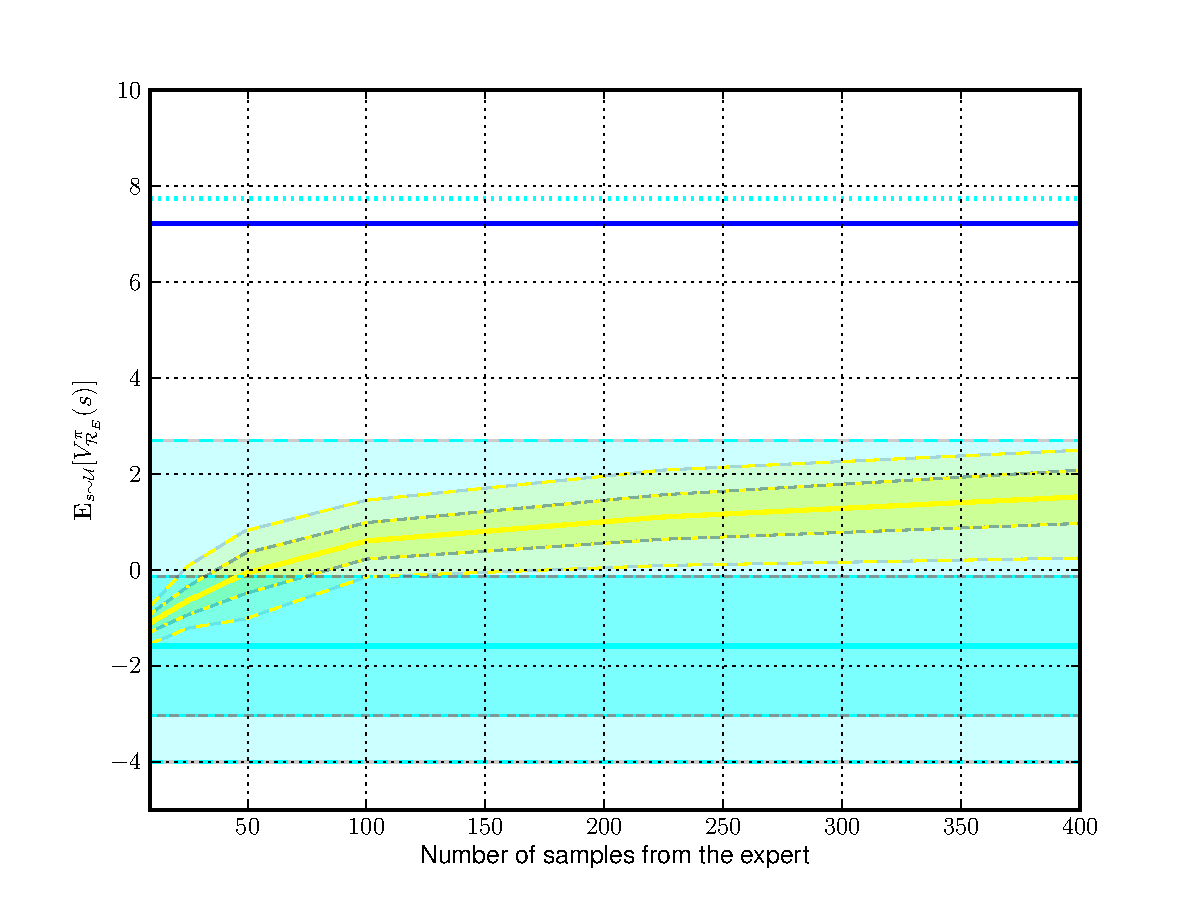
\includegraphics[width=.92\linewidth]{fig_classif.pdf}}
\end{minipage} \hfill
\begin{minipage}[r]{0.45\linewidth}
\centering
  \centerline{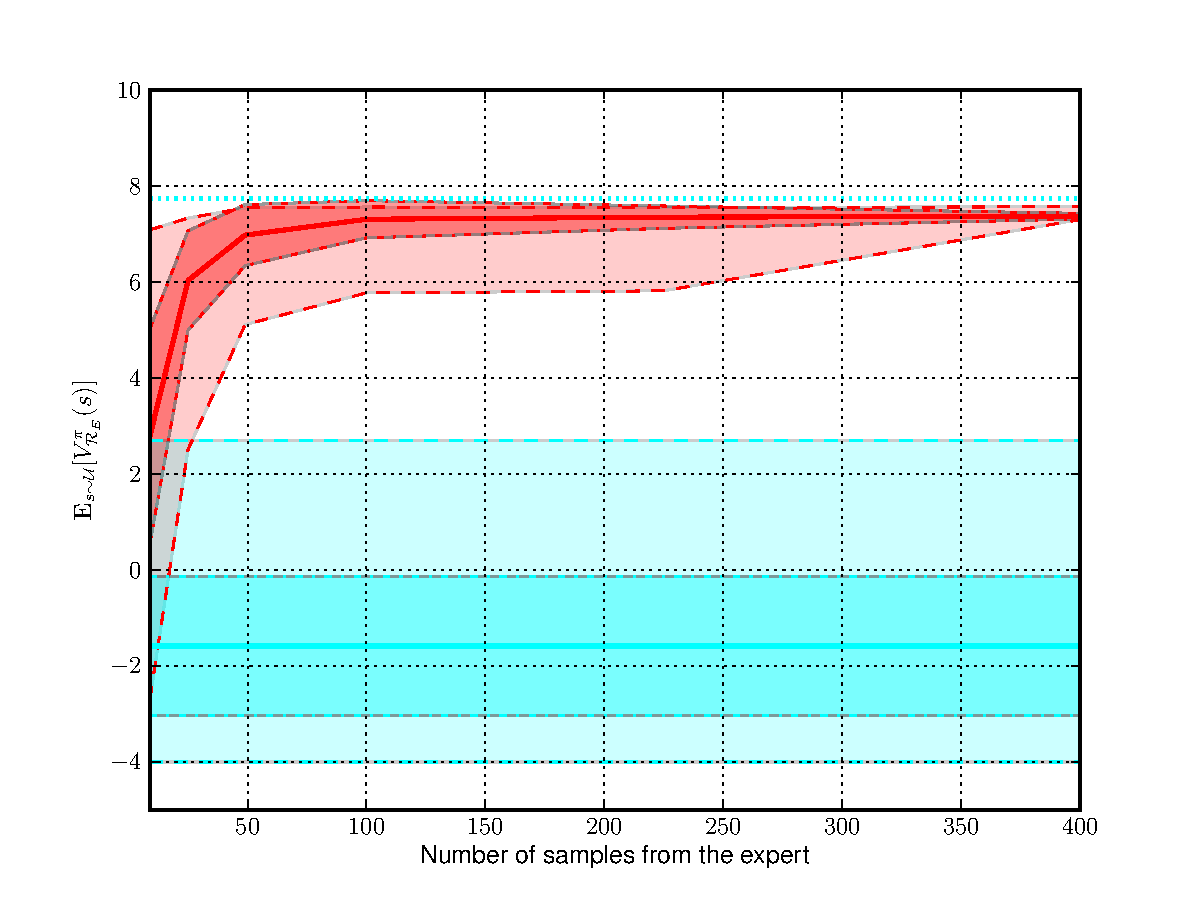
\includegraphics[width=.92\linewidth]{fig_scirl.pdf}}
\end{minipage}
\end{figure}

Fig.~\ref{fig:res} shows the performance of each approach as a
number of used expert transitions (except PIRL which uses the
model). We can see that the classifier does not work well on this
example. Increasing the number of samples would improve its
performance, but after 400 transitions it does not work as well as
SCIRL with only a ten of transitions. SCIRL works pretty well here:
after only a hundred of transitions it reaches the performance of
PIRL, both being close to the expert value. We do not report exact
computational times, but running SCIRL one time with $400$
transitions is approximately hundred time faster than running PIRL
for $70$ iteration.
%
% (this is due to the need to repeatedly solve MDPs for PIRL).

%Recall that for SCIRL the instantiation of
%Sec.~\ref{subsec:practicalApproach:instantiation} is considered,
%with a single Monte-Carlo rollout for estimating
%$\hat{\mu}^{\pi_E}(s_i,a_i)$ et using the proposed heuristic for
%$\hat{\mu}^{\pi_E}(s_i,a\neq a_i)$, which goes beyond our analysis.
%To our knowledge, it is the only algorithm working (at least on this
%benchmark) only with data from the expert.


\section{Conclusion}
\label{sec:conclusion}

We have introduced a new way to perform IRL by structuring a
linearly parameterized score function-based multi-class
classification algorithm with an estimate of the expert feature
expectation. This outputs a reward function for which we have shown
the expert to be near optimal, provided a small classification error
and a good expert feature expectation estimate. How to practically
estimate this quantity has been  discussed et we have introduced a
heuristic for the case where only transitions from the expert are
available, along with a specific instantiation of the SCIRL
algorithm. We have shown on a car driving simulator benchmark that
the proposed approach works well (even combined with the introduced
heuristic), much better than the unstructured classifier et as well
as a state-of-the-art algorithm making use of the model (and with a
much lower computational time). In the future, we plan to deepen the
theoretical properties of SCIRL (notably regarding possible
heuristics) et to apply it to real-world robotic problems.

\acknowledgements{This research was partly funded by the EU FP7 project ILHAIRE (grant
n$\deg$270780), by the EU INTERREG IVa project ALLEGRO et by the Région
Lorraine (France).}

\newpage
%\small
\bibliography{scirl_ria.bib}

\end{document} 
